\documentclass[11pt]{article}

\usepackage[a4paper]{geometry}
\geometry{left=2.0cm,right=2.0cm,top=2.5cm,bottom=2.5cm}

\usepackage{ctex} % 支持中文的LaTeX宏包
\usepackage{amsmath,amsfonts,graphicx,amssymb,bm,amsthm,mathrsfs,mathtools,breqn,subfigure} % 数学公式和符号的宏包集合
\usepackage{algorithm,algorithmicx} % 算法和伪代码的宏包
\usepackage[noend]{algpseudocode} % 算法和伪代码的宏包
\usepackage{fancyhdr} % 自定义页眉页脚的宏包
\usepackage[framemethod=TikZ]{mdframed} % 创建带边框的框架的宏包
\usepackage{fontspec} % 字体设置的宏包
\setmainfont{Times New Roman} % Set the main font to Times New Roman
\usepackage{adjustbox} % 调整盒子大小的宏包
\usepackage{fontsize} % 设置字体大小的宏包
\usepackage{tikz,xcolor} % 绘制图形和使用颜色的宏包
\usepackage{multicol} % 多栏排版的宏包
\usepackage{multirow} % 表格中合并单元格的宏包
\usepackage{pdfpages} % 插入PDF文件的宏包
\RequirePackage{listings} % 在文档中插入源代码的宏包
\RequirePackage{xcolor} % 定义和使用颜色的宏包
\usepackage{wrapfig} % 文字绕排图片的宏包
\usepackage{bigstrut,multirow,rotating} % 支持在表格中使用特殊命令的宏包
\usepackage{booktabs} % 创建美观的表格的宏包
\usepackage{circuitikz} % 绘制电路图的宏包
\usepackage{float} % Add this in the preamble
\usepackage{array}
\usepackage{physics}
\usepackage{siunitx}


\newcommand{\mm}{\unit{mm}}
\newcommand{\Hz}{\unit{Hz}}
\newcommand{\m}{\unit{m}}
\newcommand{\g}{\unit{g}}


\definecolor{dkgreen}{rgb}{0,0.6,0}
\definecolor{gray}{rgb}{0.5,0.5,0.5}
\definecolor{mauve}{rgb}{0.58,0,0.82}
\lstset{
	frame=tb,
	aboveskip=3mm,
	belowskip=3mm,
	showstringspaces=false,
	columns=flexible,
	framerule=1pt,
	rulecolor=\color{gray!35},
	backgroundcolor=\color{gray!5},
	basicstyle={\small\ttfamily},
	numbers=none,
	numberstyle=\tiny\color{gray},
	keywordstyle=\color{blue},
	commentstyle=\color{dkgreen},
	stringstyle=\color{mauve},
	breaklines=true,
	breakatwhitespace=true,
	tabsize=3,
}

% 轻松引用, 可以用\cref{}指令直接引用, 自动加前缀. 
% 例: 图片label为fig:1
% \cref{fig:1} => Figure.1
% \ref{fig:1}  => 1
\usepackage[capitalize]{cleveref}
% \crefname{section}{Sec.}{Secs.}
\Crefname{section}{Section}{Sections}
\Crefname{table}{Table}{Tables}
\crefname{table}{Table.}{Tabs.}

\setmainfont{Times New Roman}

\newcommand{\me}{\mathrm{e}}%e 指数
\newcommand{\mi}{\mathrm{i}}%虚数单位
\newcommand*{\mcelsius}{\unit{\prescript{\circ}{}C}}


\renewcommand{\emph}[1]{\begin{kaishu}#1\end{kaishu}}

%改这里可以修改实验报告表头的信息
\newcommand{\experiName}{温度的测量,用动态法测定良导体的热导率}
\newcommand{\supervisor}{梁淼}
\newcommand{\name}{徐博涵}
\newcommand{\studentNum}{2023K8009908004}
\newcommand{\class}{1}
\newcommand{\group}{04}
\newcommand{\seat}{10}
\newcommand{\dateYear}{2024}
\newcommand{\dateMonth}{10}
\newcommand{\dateDay}{21}
\newcommand{\room}{427}
\newcommand{\others}{$\square$}
%% 如果是调课、补课, 改为: $\square$\hspace{-1em}$\surd$
%% 否则, 请用: $\square$
%%%%%%%%%%%%%%%%%%%%%%%%%%%

\newcommand{\chapter}[2]{\begin{center}\bf\Large{第\,#1\,部分\quad #2}\end{center}}

\begin{document}
	
	%若需在页眉部分加入内容, 可以在这里输入
	% \pagestyle{fancy}
	% \lhead{\kaishu 测试}
	% \chead{}
	% \rhead{}
	
	\begin{center}
		\LARGE \bf 《\, 基\, 础\, 物\, 理\, 实\, 验\, 》\, 实\, 验\, 报\, 告
	\end{center}
	
	\begin{center}
		\noindent \emph{实验名称}\underline{\makebox[25em][c]{\experiName}}
		\emph{指导教师}\underline{\makebox[8em][c]{\supervisor}}\\
		\emph{姓名}\underline{\makebox[6em][c]{\name}} 
		% 如果名字比较长, 可以修改box的长度"6em"
		\emph{学号}\underline{\makebox[10em][c]{\studentNum}}
		\emph{分班分组及座号} \underline{\makebox[5em][c]{\class \ -\ \group \ -\ \seat }\emph{号}} (\emph{例}:\, 1\,-\,04\,-\,5\emph{号})\\
		\emph{实验日期} \underline{\makebox[3em][c]{\dateYear}}\emph{年}
		\underline{\makebox[2em][c]{\dateMonth}}\emph{月}
		\underline{\makebox[2em][c]{\dateDay}}\emph{日}
		\emph{实验地点}\underline{{\makebox[4em][c]\room}}
		\emph{调课/补课} \underline{\makebox[3em][c]{\others\ 是}}
		\emph{成绩评定} \underline{\hspace{5em}}
		{\noindent}
		\rule[8pt]{17cm}{0.2em}
	\end{center}	
	
\chapter{一}{动态法测定良导体的热导率}

\section{实验目的}

\begin{enumerate}
	\item 通过实验学会一种测量热导率的方法;
	\item 了解动态法的特点和优越性;
	\item 认识热波, 加强对波动理论的理解.
\end{enumerate}	


\section{实验器材}

仪器主机: 绝热材料紧裹侧表面的圆棒状样品 (本实验取铜和铝两种样品), 热电偶列阵 (传感器), 实现边界条件的脉动热源及冷却装置, 见图\ref{fig:structure measure}.

\begin{figure}[htb]
	\centering
	\subfigure[主机示意结构图1]{\includegraphics[height=4cm]{主机示意结构图1.jpg}}
	\subfigure[主机示意结构图2]{\includegraphics[height=4cm]{主机示意结构图2.jpg}}
	\caption{主机示意结构图}
	\label{fig:structure measure}
\end{figure}


温度测量: 热电偶列阵.

本实验仪器结构框图见图\ref{fig:structure measure}, 该仪器包括样品单元, 控制单元和记录单元三大部分. 本仪器由两种工作方式: 手动和程控. 他们都含样品单元和控制单元, 不同的只是记录单元: 前者用高精度 x-y记录仪; 后者用微机实现对整个系统的控制, 数据的采集, 记录和绘图.

\begin{figure}[htbp] 
	\label{fig:structure measure}
	\centering
	\includegraphics[height=6cm]{热导率动态测量仪结构框图.png}
	\caption{热导率动态测量仪结构框图}
\end{figure}


	\section{实验原理}

为使问题简化, 令热量沿一维传播, 故将样品制成棒状, 周边隔热. 取一小段样品如图\ref{fig:difx}.

\begin{figure}[!h] \label{fig:difx}
	\centering
	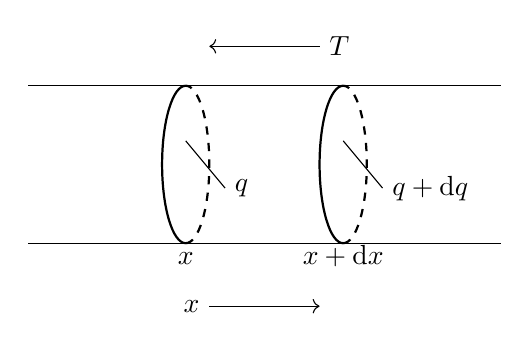
\begin{tikzpicture}
		\draw (0,0)--(6,0);
		\draw (0,2)--(6,2);
		\draw [thick] (2,2) arc (90:270:0.3 and 1);
		\draw [thick, dashed] (2,0) arc (-90:90:0.3 and 1);
		\draw [thick] (4,2) arc (90:270:0.3 and 1);
		\draw [thick, dashed] (4,0) arc (-90:90:0.3 and 1);
		\draw [<-] (2.3,2.5)--(3.7,2.5) node[right]{$ T $};
		\draw [->] (2.3,-0.8) node[left]{$ x $}--(3.7,-0.8);
		\node [below] at(2,0) {$ x $};
		\node [below] at(4,0.1) {$ x+\dd{x} $};
		\draw (2,1.3)--(2.5,0.7) node[right]{$ q $};
		\draw (4,1.3)--(4.5,0.7) node[right]{$ q+\dd{q} $};
	\end{tikzpicture}
	\caption{棒元示意图}
\end{figure}


根据热传导定律, 单位时间内流过某垂直于传播方向上面积A 的热量, 即热流为:
\[
\pdv {q}{t} = -kA \pdv {T}{x}
\]
其中$k$为待测材料的热导率, $A$为截面积, 文中$\pdv Tx$是温度对坐标$x$的梯度. 两边对坐标取微分有:
\[
\dd{\pdv {q}{t}} = -kA \pdv[2]{T}{x}\dd{x}
\]
据能量守恒定律, 任一时刻棒元的热平衡方程为:
\[
C\rho A\dd{x}\pdv {T}{t} = \dd{\pdv{q}{t}}  = -kA \pdv[2]{T}{x}\dd {x}
\]
其中$C,\rho$分别为材料的比热容与密度, 由此可得热流方程:
\[
\pdv {T}{t} = D\pdv[2]{T}{x}
\]
其中$D = \dfrac{k}{C\rho}$, 称为热扩散系数.

对于这个偏微分方程, 在初始条件为恒温的情况下, 根据不同的边界条件可以给出不同的确定的解. 实验中, 令热端的温度按简谐变化如$T = T_0 + T_{\mathrm{m}}\sin\omega t$, 另一端用凉水冷却, 保持恒定低温$T_0$, 那么可以给出棒中各点的温度:
\[
T = T_0 - \alpha x + T_{\mathrm{m}} \mathrm{e}^{-\sqrt{\frac{\omega}{2D}}x} \cdot \sin \left( \omega t - \sqrt{\frac{\omega}{2D}}x \right)
\]
其中$T_0$是直流成分, $\alpha$是线性成分的斜率. 可以看出:

热端(x=0)处温度按简谐方式变化时, 这种变化将以衰减波的形式在棒内向冷端传播, 称为热波. 热波的波速和波长如下:
\begin{gather*}
	v = \sqrt{2D\omega}\\
	\lambda = 2\pi\sqrt{\frac{2D}{\omega}}
\end{gather*}
因此在热端温度变化的角频率$\omega$已知的情况下, 只要测出波速或波长就可以计算出$D$, 然后再由计算出材料的热导率$k$. 本实验采用波速计算, 可得:
\[
v^2 = \frac{2k\omega}{C\rho} \quad\Longrightarrow\quad k = \frac{v^2C\rho}{4\pi f} = \frac{v^2C\rho T}{4\pi}
\]
其中, $f,T$分别为热端温度按简谐变化的频率和周期. 根据这个公式, 我们就可以使用测得的数据来计算热导率$k$.

\section{实验内容及注意事项}

测量铜棒和铝棒的导热率. (先测铜棒后测铝棒) 

\begin{enumerate}
	
	\item 实验前, 检查管路是否堵塞. 打开仪器盖, 仔细阅读注意事项. 两端冷却水管在两个样品中是串连的, 水流先走铝后走铜. (一般先测铜样品, 后测铝样品, 以免冷却水变热.)
	
	\item 打开水源, 从出水口观察流量, 要求水流稳定 (将阀门稍微打开即可).
	
	\begin{enumerate}
		
		\item (热端水流量较小时, 待测材料内温度较高; 水流较大时, 温度波动较大.) 因此热端水流要保持一个合适的流速, 阀门开至1/3开度即可. 冷端水流量要求不高, 只要保持固定的室温即可. 
		
		\item 调节水流: 保持电脑操作软件的数据显示曲线幅度和形状较好.
		
		\item 实际上不用冷端冷却水也能实验, 只是需要很长时间样品温度才能动态平衡. 而且环境温度变化会影响测量. 
		
	\end{enumerate}
	
	\item 打开电源开关, 主机进入工作状态, 选择 "程控" 工作方式开始测量.
	
	\begin{enumerate}
		
		\item 完成前述实验步骤, 调节好合适的水流量. 因进水电磁阀初始为关闭状态, 需要在测量开始后加热器停止加热的半周期内才调整和观察热端流速. 
		
		\item 打开操作软件. 操作软件使用方法参见实验桌内的 "实验指导" 中 "操作软件使用" 部分说明.
		
		\item "平滑" 功能尽量不要按, 防止信号失真. 
	\end{enumerate}
	
	\item 在控制软件中设置热源周期$T = 180\unit{s}$. 选择铜样品进行测量. 
	
	\item 设置$x,y$轴单位坐标. $x$方向为时间, 单位是秒, $y$方向是信号强度, 单位为毫伏 (与温度对应). 
	
	\item 在 "选择测量点" 栏中选择一个或某几个测量点. 
	
	\item 按下 "操作" 栏中 "测量" 按钮, 仪器开始测量工作, 在电脑屏幕上画出$T$-$t$曲线簇. $40$分钟后, 系统进入动态平衡, 样品内温度动态稳定. 此时按下 "暂停" , 在 "文件" 菜单中选择保存, 存储数据.
	
	\item 换用铝样品, 重复上几个步骤, 继续测量.
	
	\item 将实验数据通过网络发送给实验人供存储用. 实验结束后, 按顺序先关闭测量仪器, 然后关闭自来水, 最后关闭电脑. 
	
\end{enumerate}

\textbf{实际上本实验同学需要做的是:}
\begin{enumerate}
	\item 打开所有水龙头,阀门打开至1/3处.\newline
	\textbf{由于教室中所有的仪器冷却水均串联,故不好判断水池中哪些水管是无用的,因此为了实验安全,将所有水龙头打开}.
	\item 打开电脑上的测量程序,检查参数无误后开始运行.
	\item 待测量数据稳定后输出,在数据中寻找峰值.\newline
	\textbf{为了方便后续的读出,最好将数据输出为excel格式}.\newline
	\textbf{由于只需要记录6组数据,因此若有一个探测器数据损坏,则可以隔项将这组数据跳过,可见图\ref{fig:wrong sensor}}.
	\begin{figure}
		\centering
		\includegraphics[height=5cm]{错误的热导率测量数据.png}
		\caption{红框中的数据出现错误,于是将其忽略并选取1,3,5,7,9,11组的数据}
		\label{fig:wrong sensor}
	\end{figure}
	\item 等待所有数据测量均结束后再关闭水龙头.\newline
	\textbf{由于冷却水串联,需要确保所有同学均完成后再共同关闭冷却水}.
\end{enumerate}

\section{实验结果与数据处理}
已知:相邻热电偶的间距$ l_0=2\,\mathrm{cm} $, 周期$ T=180\,\mathrm{s} $, 铜的比热为$ 0.385\,\mathrm{J/(g\cdot K)} $, 密度为$ 8.92\,\mathrm{g/m^3} $; 铝的比热为$ 0.880\,\mathrm{J/(g\cdot K)} $, 密度为$ 2.7\,\mathrm{g/cm^3} $. 
\subsection{铜样品的热导率}

可使用计算公式如下:
\[
k = \frac{v^2C\rho T}{4\pi}
\]

代入合适单位后, 可得数据值如表\ref{tab:Cu},其中,三组波速数据利用逐差法求出:
\begin{table}[htbp]
	\centering
	\begin{tabular}{|lll|llll|}
		\hline
		\multicolumn{1}{|l|}{测量点n}                           & \multicolumn{1}{l|}{1}       & 3       & \multicolumn{1}{l|}{5}       & \multicolumn{1}{l|}{7}       & \multicolumn{1}{l|}{9}       & 11      \\ \hline
		\multicolumn{1}{|l|}{对应峰值时间$t (\mathrm{s})$}                    & \multicolumn{1}{l|}{1541.42} & 1556.04 & \multicolumn{1}{l|}{1570.52} & \multicolumn{1}{l|}{1582.52} & \multicolumn{1}{l|}{1591.04} & 1599.52 \\ \hline
		\multicolumn{1}{|l|}{波速 $v (\num{e-3} \mathrm{m/s})$} & \multicolumn{1}{l|}{2.92}    & 3.43    & \multicolumn{1}{l|}{4.13}    & \multicolumn{1}{l|}{}        & \multicolumn{1}{l|}{}        &         \\ \hline
		\multicolumn{3}{|l|}{波速平均值:$\num{3.49e-3} \mathrm{m/s}$}                                                              & \multicolumn{4}{l|}{热导率:$599.15 \mathrm{W/m \cdot K}$}                                                                \\ \hline
	\end{tabular}
	\caption{铜热导率数据记录表}
	\label{tab:Cu}
\end{table}



\subsection{铝样品的热导率}

同上, 铝样品的结果如表\ref{tab:Al},波速数据同样用逐差法求出:

\begin{table}[htbp]
	\centering
	\begin{tabular}{|lll|llll|}
		\hline
		\multicolumn{1}{|l|}{测量点n}                           & \multicolumn{1}{l|}{1}       & 2       & \multicolumn{1}{l|}{3}       & \multicolumn{1}{l|}{4}       & \multicolumn{1}{l|}{5}       & 6      \\ \hline
		\multicolumn{1}{|l|}{对应峰值时间$t (\mathrm{s})$}                    & \multicolumn{1}{l|}{3517.52} & 3524.04 & \multicolumn{1}{l|}{3535.04} & \multicolumn{1}{l|}{3542.04} & \multicolumn{1}{l|}{3552.04} & 3560.04 \\ \hline
		\multicolumn{1}{|l|}{波速 $v (\num{e-3} \mathrm{m/s})$} & \multicolumn{1}{l|}{2.45}    & 2.14    & \multicolumn{1}{l|}{2.40}    & \multicolumn{1}{l|}{}        & \multicolumn{1}{l|}{}        &         \\ \hline
		\multicolumn{3}{|l|}{波速平均值:$\num{2.33e-3} \mathrm{m/s}$}                                                              & \multicolumn{4}{l|}{热导率:$184.77 \mathrm{W/m \cdot K}$}                                                                \\ \hline
	\end{tabular}
	\caption{铝热导率数据记录表}
	\label{tab:Al}
\end{table}

\section{思考题}

\begin{enumerate}
	
	\item 如果想知道某一时刻$t$时材料棒上的热波, 即$T$-$x$曲线, 将如何做? 
	
	取同一时刻的热波测量点,即得到$T$-$x$曲线
	
	\item 为什么较后面测量点的$T$-$t$曲线振幅越来越小? 
	
	由实验原理中的温度公式:
	\[
	T = T_0 - \alpha x + T_{\mathrm{m}} \mathrm{e}^{-\sqrt{\frac{\omega}{2D}}x} \cdot \sin \left( \omega t - \sqrt{\frac{\omega}{2D}}x \right)
	\]
	由于存在衰减因子$\mathrm{e}^{-\sqrt{\frac{\omega}{2D}}x}$,因此$x$越大,振幅越小.
	
	\item 为什么实验中铝棒的测温点才$8$个, 而铜棒的测温点达到$12$个? 
	
	铜的热导率较高,因此传热速度更快,相邻的两个测量点之间差距更小,因此需要更多的数据点来减小误差.
	
	\item 实验中误差的来源有哪些? 
	\begin{enumerate}
		\item \textbf{在推导过程中,认为热端的温度按简谐变化,但是在实验中,热端的加热实际上是按方波进行,因此热端温度并不是严格的简谐变化,因而会出现很多数据“叠在一起”的峰值区域.}
		\item 由于仪器中铜棒和铝棒被反复加热,且没有利用砂纸摩擦,可能会导致表面氧化,导致热导率变化.
		\item 仪器精度不高,难以精确测量峰值时间
	\end{enumerate}

	
\end{enumerate}

\newpage
\setcounter{section}{0}

\chapter{二}{温度的测量和温度计的设计}





\section{实验目的}

\begin{enumerate}
	
	\item 用电位差计测热电偶的温差电动势;
	
	\item 用平衡电桥测热敏电阻和铜电阻的电阻值;
	
	\item 设计非平衡电桥实现对热敏电阻的实时测量.
	
\end{enumerate}




\section{实验器材}
为进行温度计的控温,我们采用DHT-2型热学实验仪,其前面板见图\ref{fig:3},这个装置中含有热电偶,铜电阻以及热敏电阻,并有加热炉和风扇进行升温和降温.

\begin{figure}[htbp]
	\centering
	\includegraphics[width=8cm]{图3.jpg}
	\caption{DHT-2型热学实验仪的前面板示意图}
	\label{fig:3}
\end{figure}

为测量热电偶的电压,我们采用UJ36a型携带式直流电位差计,其电路图和操作面板分别见图\ref{fig:4}和图\ref{fig:5}:

\begin{figure}[htbp]
	\centering
	\includegraphics[width=8cm]{图4.jpg}
	\caption{UJ36a型携带式直流电位差计的补偿法电路图}
	\label{fig:4}
\end{figure}

\begin{figure}[htbp]
	\centering
	\includegraphics[width=8cm]{图5.jpg}
	\caption{UJ36a型携带式直流电位差计的操作面板示意图}
	\label{fig:5}
\end{figure}

为了利用平衡电桥测热敏电阻和铜电阻的电阻值,我们采用DHQJ-5型教学用多功能电桥,其电路图和操作面板分别见图\ref{fig:6}和图\ref{fig:7}:

\begin{figure}[htbp]
	\centering
	\includegraphics[width=8cm]{图6.jpg}
	\caption{DHQJ-5型教学用多功能电桥的补偿法电路图}
	\label{fig:6}
\end{figure}

\begin{figure}[htbp]
	\centering
	\includegraphics[width=8cm]{图7.jpg}
	\caption{DHQJ-5型教学用多功能电桥的操作面板示意图}
	\label{fig:7}
\end{figure}







\section{实验原理}

\subsection{电位差计测热电偶温差电动势}
当两种不同材料1,B的金属丝端点相互接触且端点处温度不同时,整个回路就会产生温差电动势,并且有近似关系式:\[E_x=\alpha(t-t_0)\]其中$E_x$为温差电动势,$t-t_0$为温差\newline

注意,为了测量回路中的温差电动势,我们需要接入一种新的材料C,但是若端点处温度不同,会改变原回路的电动势,为了避免这种情况,需要将新接入的两个端点全部浸入冰水混合物中.
\begin{figure}[htbp]
	\centering
	\includegraphics[height=3.5cm]{热电偶温度计.jpg}
	\caption{新接入的两个端点全部浸入冰水混合物中}
	\label{fig:冰水混合物}
\end{figure}

\subsection{用平衡电桥测电阻的温度特性曲线}
\subsubsection{铜电阻}
当温度在室温附近时,铜电阻的电阻值随温度的变化可以描述为:\[R_x=R_0(1+\alpha t)\],利用DHT-2型热学实验仪改变铜电阻的温度,再利用电桥测出铜电阻的阻值,即可得到铜电阻的温度特性曲线,线性拟合得到温度系数.
\subsubsection{热敏电阻}
热敏电阻的温度特性为:
\begin{displaymath}
	R_T=A e^{\frac{B}{T}}
\end{displaymath}
求拟合时,在等式两侧取$\ln$:
\begin{displaymath}
	\ln R_T=\ln A+\frac{B}{T}
\end{displaymath}

\subsection{利用非平衡电桥和热敏电阻制作温度计}
我们认为电压表内阻无穷大而忽略通过电压表的电流,这样就可以求出$U_0$:\begin{displaymath}U_0=\left( \frac{R_x}{R_2+R_x}+\frac{R_3}{R_1+R_3}\right)E\end{displaymath}其中$R_x=A\exp \left(\frac{B}{T}\right)$,我们将其代入并进行Taylor级数展开,忽略三阶以上的小量就得到了线性的关系式:\begin{displaymath}U_0=\lambda+m(t-t_1)\end{displaymath}其中,\begin{displaymath}\lambda=\left(\frac{B+2T_1}{2B}-\frac{R_3}{R_1+R_3}\right)E,m=\left(\frac{4T_1^2-B^2}{4BT_1^2}\right)E\end{displaymath}成立。

这样就可以得到:\begin{displaymath}E=\left(\frac{4BT_1^2}{4T_1^2-B^2}\right)m,\quad R_2=\frac{B-2T}{B+2T}R_{xT_1},\quad \frac{R_1}{R_3}=\frac{2BE}{(B+2T_1)E-2B\lambda}-1\end{displaymath}
设定好理论值后还需要调整参数,例如将控温仪温度设置在40\mcelsius,微调$R_2$,使得电压接近-400mV






\section{实验内容及注意事项}

\begin{enumerate}
	\item 开启温控仪电源,给热端加热,在 30℃至 50℃区间,每隔5\mcelsius 测一组数据,需要注意:
	
	\begin{enumerate}
		\item 等待温度稳定后再进行测量
		\item \textbf{由于反复升温降温较为复杂,故当加热到同一温度处应同时测量热电偶,铜电阻和热敏电阻的数据}
		\item \textbf{本次实验的一个难点在于难以精确控制温度,没有办法将温度保持恒定在我们需要测量的温度,实践发现当温度上升到距离指定温度0.5\mcelsius 时就打开风扇,可以使其在指定温度处停留较长时间.}
	\end{enumerate}
	\item 选定$\lambda=400\mathrm{mV},\quad m=-10\mathrm{mV/\mcelsius},\quad t_1=40\mcelsius$,根据实验原理中的公式进行计算并微调,再测几组数据,用于测试自己设计的温度计的精度.
\end{enumerate}





\section{实验结果与数据处理}
	
	\subsection{用电位差计测热电偶温差电动势}
	
	实验数据如表\ref{tab:热电偶},室温$t=24\mcelsius$,电动势$E_x=0.47\mathrm{mV}$,冷端温度$t_0=0\mcelsius$
	% Table generated by Excel2LaTeX from sheet '非平衡电桥热敏电阻温度计的设计'
	\begin{table}[htbp]
		\centering
		\caption{热电偶温差电动势与温度差关系}
		\begin{tabular}{|l|l|r|r|r|r|r|}
			\hline
			热端温度 $t$   & $\mcelsius$  & 30.0    & 35.0    & 40.0    & 44.9    & 50.0  \bigstrut\\
			\hline
			电动势 $E_x$   & $\unit{mV}$ & 0.85   & 1.06   & 1.23   & 1.40   & 1.61  \bigstrut\\
			\hline
		\end{tabular}%
		\label{tab:热电偶}%
	\end{table}%
	
	利用公式$E_x=\alpha(t-t_0)$,对$\alpha$进行拟合,拟合图像见图\ref{fig:热电偶},得到$\alpha=0.0373$.
	\begin{figure}[htbp]
		\centering
		\includegraphics[height=3.5cm]{热电偶温差电系数.png}
		\caption{拟合结果$\alpha=0.0373$}
		\label{fig:热电偶}
	\end{figure}
	
	作图和拟合所用的mathematica代码如下
	\begin{lstlisting} 
		ClearAll["Global`*"]
		data1 = {{30.0, 0.85}, {35.0, 1.06}, {40.0, 1.23}, {44.9, 
				1.40}, {50.0, 1.61}}
		fitpara1 = FindFit[data1, a*x + b, {a, b}, x]
		fitted1 = a x + b /. fitpara1
		
		Show[{Plot[fitted1, {x, 30, 50}, 
			AxesLabel -> {"热端温度 t (°C)", "电动势 (mV)"}, PlotStyle -> Red]
			, ListPlot[data1]}]
	\end{lstlisting}
	
	
	
	\subsection{平衡电桥测铜电阻温度特性曲线}
	实验数据如表\ref{tab:铜电阻},室温$t=24.4\mcelsius$,电阻$R_T=57.4\Omega$.
	\begin{table}[htbp]
	\centering
	\caption{平衡电桥测铜电阻温度特性曲线}
	\begin{tabular}{|l|l|r|r|r|r|r|}
		\hline
		热端温度 $t$   & $\mcelsius$  & 30.0    &   35.0    & 40.0    & 44.9    & 50.0  \bigstrut\\
		\hline
		电动势 $E_x$   & $\unit{mV}$ & 58.6   & 59.8   & 60.7   & 61.7   & 62.8  \bigstrut\\
		\hline
	\end{tabular}%
	\label{tab:铜电阻}%
	\end{table}%
	
	利用公式$R_x=R_0(1+\alpha t)$,对$\alpha$进行拟合,拟合图像见图\ref{fig:铜电阻},得到$\alpha=0.0039$.
	
	\begin{figure}[htbp]
	\centering
	\includegraphics[height=3.5cm]{铜电阻温度系数.png}
	\caption{拟合结果$\alpha=0.0039$}
	\label{fig:铜电阻}
	\end{figure}
	
	
	
	\subsection{平衡电桥测热敏电阻温度特性曲线}
	实验数据如表\ref{tab:热敏电阻},室温$t=24.4\mcelsius$,电阻$R_T=2728.2\Omega$.

	\begin{table}[htbp]
		\centering
		\caption{平衡电桥测热敏电阻温度特性曲线}
		\begin{tabular}{|l|l|r|r|r|r|r|}
			\hline
			热端温度 $t$   & $\mcelsius$  & 29.8    &   35.0    & 40.0    & 44.9    & 50.0  \bigstrut\\
			\hline
			电动势 $E_x$   & $\unit{mV}$ & 2182.0   & 1776.7   & 1462.9   & 1204.0   & 993.7  \bigstrut\\
			\hline
		\end{tabular}%
		\label{tab:热敏电阻}%
	\end{table}%
	
	利用公式$R_T=A e^{\frac{B}{T}}$,对A和B进行拟合,拟合图像见图\ref{fig:热敏电阻},得到$A=0.00754\quad B=3811.2$.
	\begin{figure}[htbp]
		\centering
		\includegraphics[height=3.5cm]{热敏电阻.png}
		\caption{拟合结果:A=0.00754,B=3811.2}
		\label{fig:热敏电阻}
	\end{figure}
	
	
	
	\subsection{非平衡电桥热敏电阻温度计的设计}
	利用“平衡电桥测热敏电阻温度特性曲线”得到的数据,代入公式
	
	\begin{displaymath}E=\left(\frac{4BT_1^2}{4T_1^2-B^2}\right)m,\quad R_2=\frac{B-2T}{B+2T}R_{xT_1},\quad \frac{R_1}{R_3}=\frac{2BE}{(B+2T_1)E-2B\lambda}-1\end{displaymath}
	可以解得
	\begin{equation*}
		E=1.06\mathrm{V},\quad R_2=1049.95\Omega,\quad  
		\frac{R_1}{R_3}=0.0413
	\end{equation*}
	将控温仪温度设置在40\mcelsius,微调$R_2$,使得电压接近-400mV,微调后的实际值:
	\begin{equation*}
		R_1=41.3\Omega,\quad R_2=1049.5\Omega,\quad  
		R_3=1000\Omega
	\end{equation*}
	微调后,对温度计进行测试,调整设定温度为40\mcelsius 至 50\mcelsius,记录温度计读出的数据于表\ref{tab:温度计}:
	\begin{table}[htbp]
		\centering
		\caption{温度计测试数据}
		\begin{tabular}{|l|l|r|r|r|r|r|}
			\hline
			设定温度$t$ & $\mcelsius$ & 39.9    & 42.5    & 45.0    & 47.5    & 50.0  \bigstrut\\
			\hline
			测试电压$U_0$ & mV      & -400  & -425  & -449  & -474  & -498  \bigstrut\\
			\hline
			测试温度    & $\mcelsius$ & 40.0    & 42.5    & 44.9    & 47.4    & 49.8  \bigstrut\\
			\hline
		\end{tabular}%
		\label{tab:温度计}%
	\end{table}%
	
	作图,拟合及计算数据所用的mathematica代码如下
	\begin{lstlisting}
		ClearAll["Global`*"]
		T1 = 40 + 273.15;
		f[R_] := Log[R];
		g[T_] := 1/(T + 273.15);
		
		data = {{g[29.8], f[2182.0]}, {g[35.0], f[1776.7]}, {g[40.0], 
				f[1462.9]}, {g[45.0], f[1204.0]}, {g[50.0], f[993.7]}};
		
		fitpara = FindFit[data, B*x + F, {B, F}, x];
		{B, A} = {B, Exp[F]} /. fitpara
		fitted = A*Exp[B/x]
		data123 = {{29.8 + 273.15, 2182.0}, {35.0 + 273.15, 
				1776.7}, {40.0 + 273.15, 1462.9}, {45.0 + 273.15, 
				1204.0}, {50.0 + 273.15, 993.7}};
		Show[{Plot[fitted, {x, 30 + 273.15, 50 + 273.15}, 
			AxesLabel -> {"温度 T (K)", "电阻 (\[CapitalOmega])"}, 
			PlotStyle -> Red, PlotLabel -> "平衡电桥测热敏电阻温度特性曲线"], 
			ListPlot[data123]}]
		
		e = ((4*B*T1^2)/(4 T1^2 - B^2))*(-0.01)
		R2 = (B - 2 T1)/(B + 2 T1)*1462.9
		R1/R3 = (2 B*e)/((B + 2 T1) e - 2 B*(-0.4)) - 1
	\end{lstlisting}
	
	
	
	
	
	\section{实验感想}
	本次实验我认为还是比较轻松的,比较困难的一点是在课上就要求对数据进行拟合,需要同学们熟练掌握数据处理的方法,如果提前学习了Excel或mathematica这样的软件就可以做到事半功倍.另外在设计温度计的部分需要做好预习报告,尤其需要看懂推导过程,理解温度计的设计原理,否则即使操作熟练也可能会无从下手.
	
	另外,由于其中考试,实验报告上交的比较迟,十分抱歉.
	
	
	
	
	\section{原始数据记录表}
	
		\includepdf[pages={1-2}]{温度测量实验原始记录表.pdf}
	
	
\end{document}